\section{Introduction}
\label{sec:intro}
% MAKE IT VERY CLEAR THAT WE WANT TO RESEARCH EASIER METHODS THAN ACTOR CRITIC FOR SOLVING THE PROBLEM

% Reinforcement learning has previously been used to solve a number of different games such as Chess\footnote{\href{https://arxiv.org/pdf/1712.01815.pdf}{Mastering Chess and Shogi by Self-Play with a General Reinforcement Learning Algorithm}} and Go\footnote{\href{https://www.nature.com/articles/nature24270.epdf}{Mastering the game of Go without human knowledge}}, both of which are zero sum games. Reinforcement learning has excelled at playing Go, where the number of possible moves are so many that a traditional heuristic is not sufficient to solve the problem successfully. These games only contain two players, whereas a game like Dota II is 5 vs. 5 game. That makes it a multi-agent environment and a non-zero sum game, which introduces additional challenges for machine learning.\footnote{\href{https://blog.openai.com/openai-five/}{OpenAI Five}}

\emph{\say{Accomplishing tasks with infinitely meaningful variation is common in the real world and difficult to simulate.}}\cite{pommerman} One place where this can be simulated is in games. Reinforcement learning has in recent years been utilised to solve a number of games such as Go\cite{silver2017masteringgo}\cite{silver2016a}, chess\cite{silver2017masteringchess} and many others\cite{mnih2015a}. In the game of Go does the number of possible moves by far exceeds the capabilities of a traditional heuristic, but reinforcement learning has shown to be excellent for training an agent to solve the problem of playing and winning the game successfully.\cite{silver2017masteringgo} The huge amount of unique states in Go is similar to the game of Pommerman, which is a variation of the original Bomberman developed by Hudson soft. in 1983. In Pommerman is every game played on a new random generated board, as seen in figure~\ref{fig:pomIntro} and the game can be played as a Free For All (FFA) or as in teams of two.\cite{pommerman} The random boards and the four players moving independently of each other are the reasons for the vast number of possible states in the game.

\begin{figure}[htb]
    \centerline{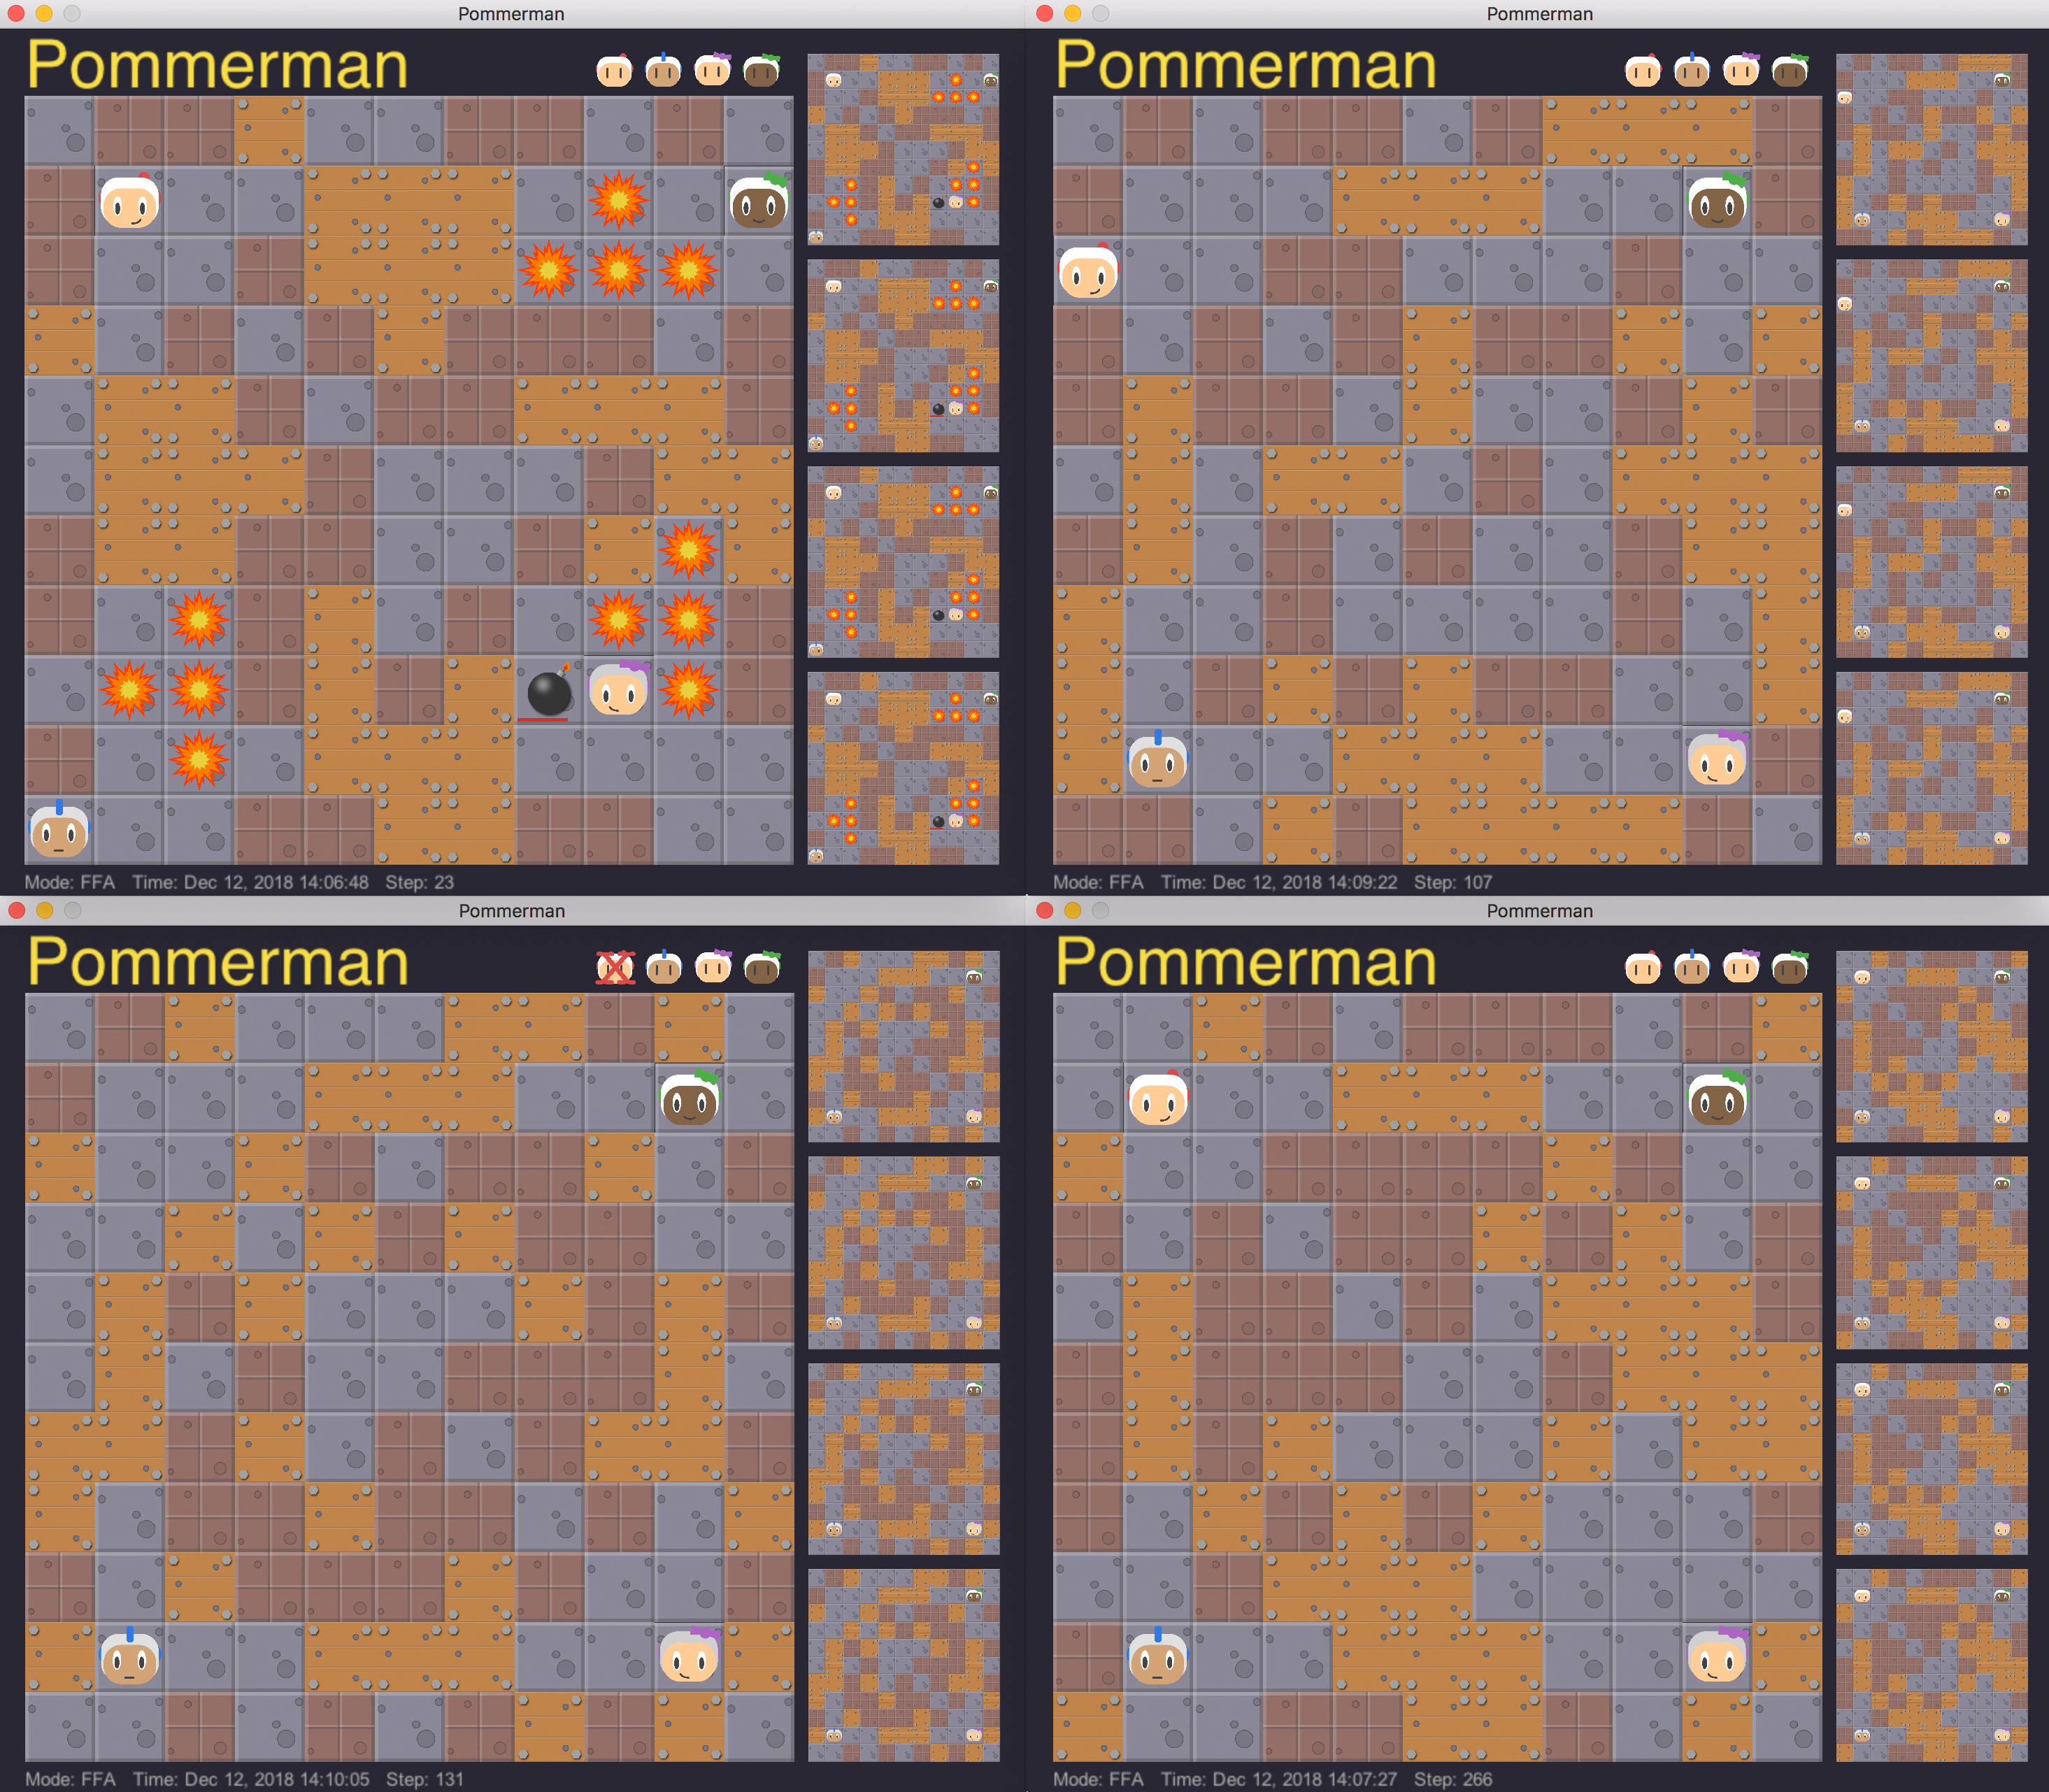
\includegraphics[width=0.7\linewidth]{docs/article/inputs/4pommerview.jpg}}
    \caption{Four random boards in typical games of Pommerman.}
    \label{fig:pomIntro}
\end{figure}

In the FFA version of Pommerman has the actor-critic algorithm shown to be performing very well.\cite{rwightman} The goal in this paper is to research if other more simple deep reinforcement learning algorithms can be utilised to solve the problem of training an agent to play the FFA Pommerman against so called random and simple agents, with similar or better performance than what is the result of \cite{rwightman}. The motivation for doing so... INSERT MOTIVATION HERE

% Motivation
% The motivation for researching state of the art techniques for solving these problems is intriguing. Although much research has been done in the past years we have not yet seen revolutionary approaches, making headline such as AlphaZero or AlphaGo. We as a group would like to explore these state of the art approaches on the game Pommerman to evaluate how far machine learning has come, solving non-zero sum games in single- and multi-agent environments. We do not strafe for ground breaking research within the topic.

% Give an overview of the article, section by section
In section~\ref{sec:relatedwork}, are related works presented. In section~\ref{sec:methods} are the different algorithms described as well as implemented features to restrict the complexity of the problem and increase the performance of the agent. In section~\ref{sec:results} are the results of the implements methods shown. In section~\ref{sec:discussion} are the issues faced during the research discussed. In section~\ref{sec:futurework} will it be covered what techniques and algorithms should be investigated in future work. Finally is the paper concluded in section~\ref{sec:conclusion}.